\cleardoublepage
\chapter*{Appendix}
%{\usekomafont{section} Appendix}
First Backmatter stuff.


%%%%%%%%%%% TBP on Ag(100) @ RT - single ordered island
\paragraph{Ordered areas}
Only a single ordered area of TBP on Ag(100) was found, but its structure could not be resolved properly due to tip issues (compare figure \ref{fig:hex-TBP-Ag100}). Its unit cell looks hexagonal with roughly \SI{1.7} {\nano \meter} period. 

\begin{figure}[h]
	\centering
	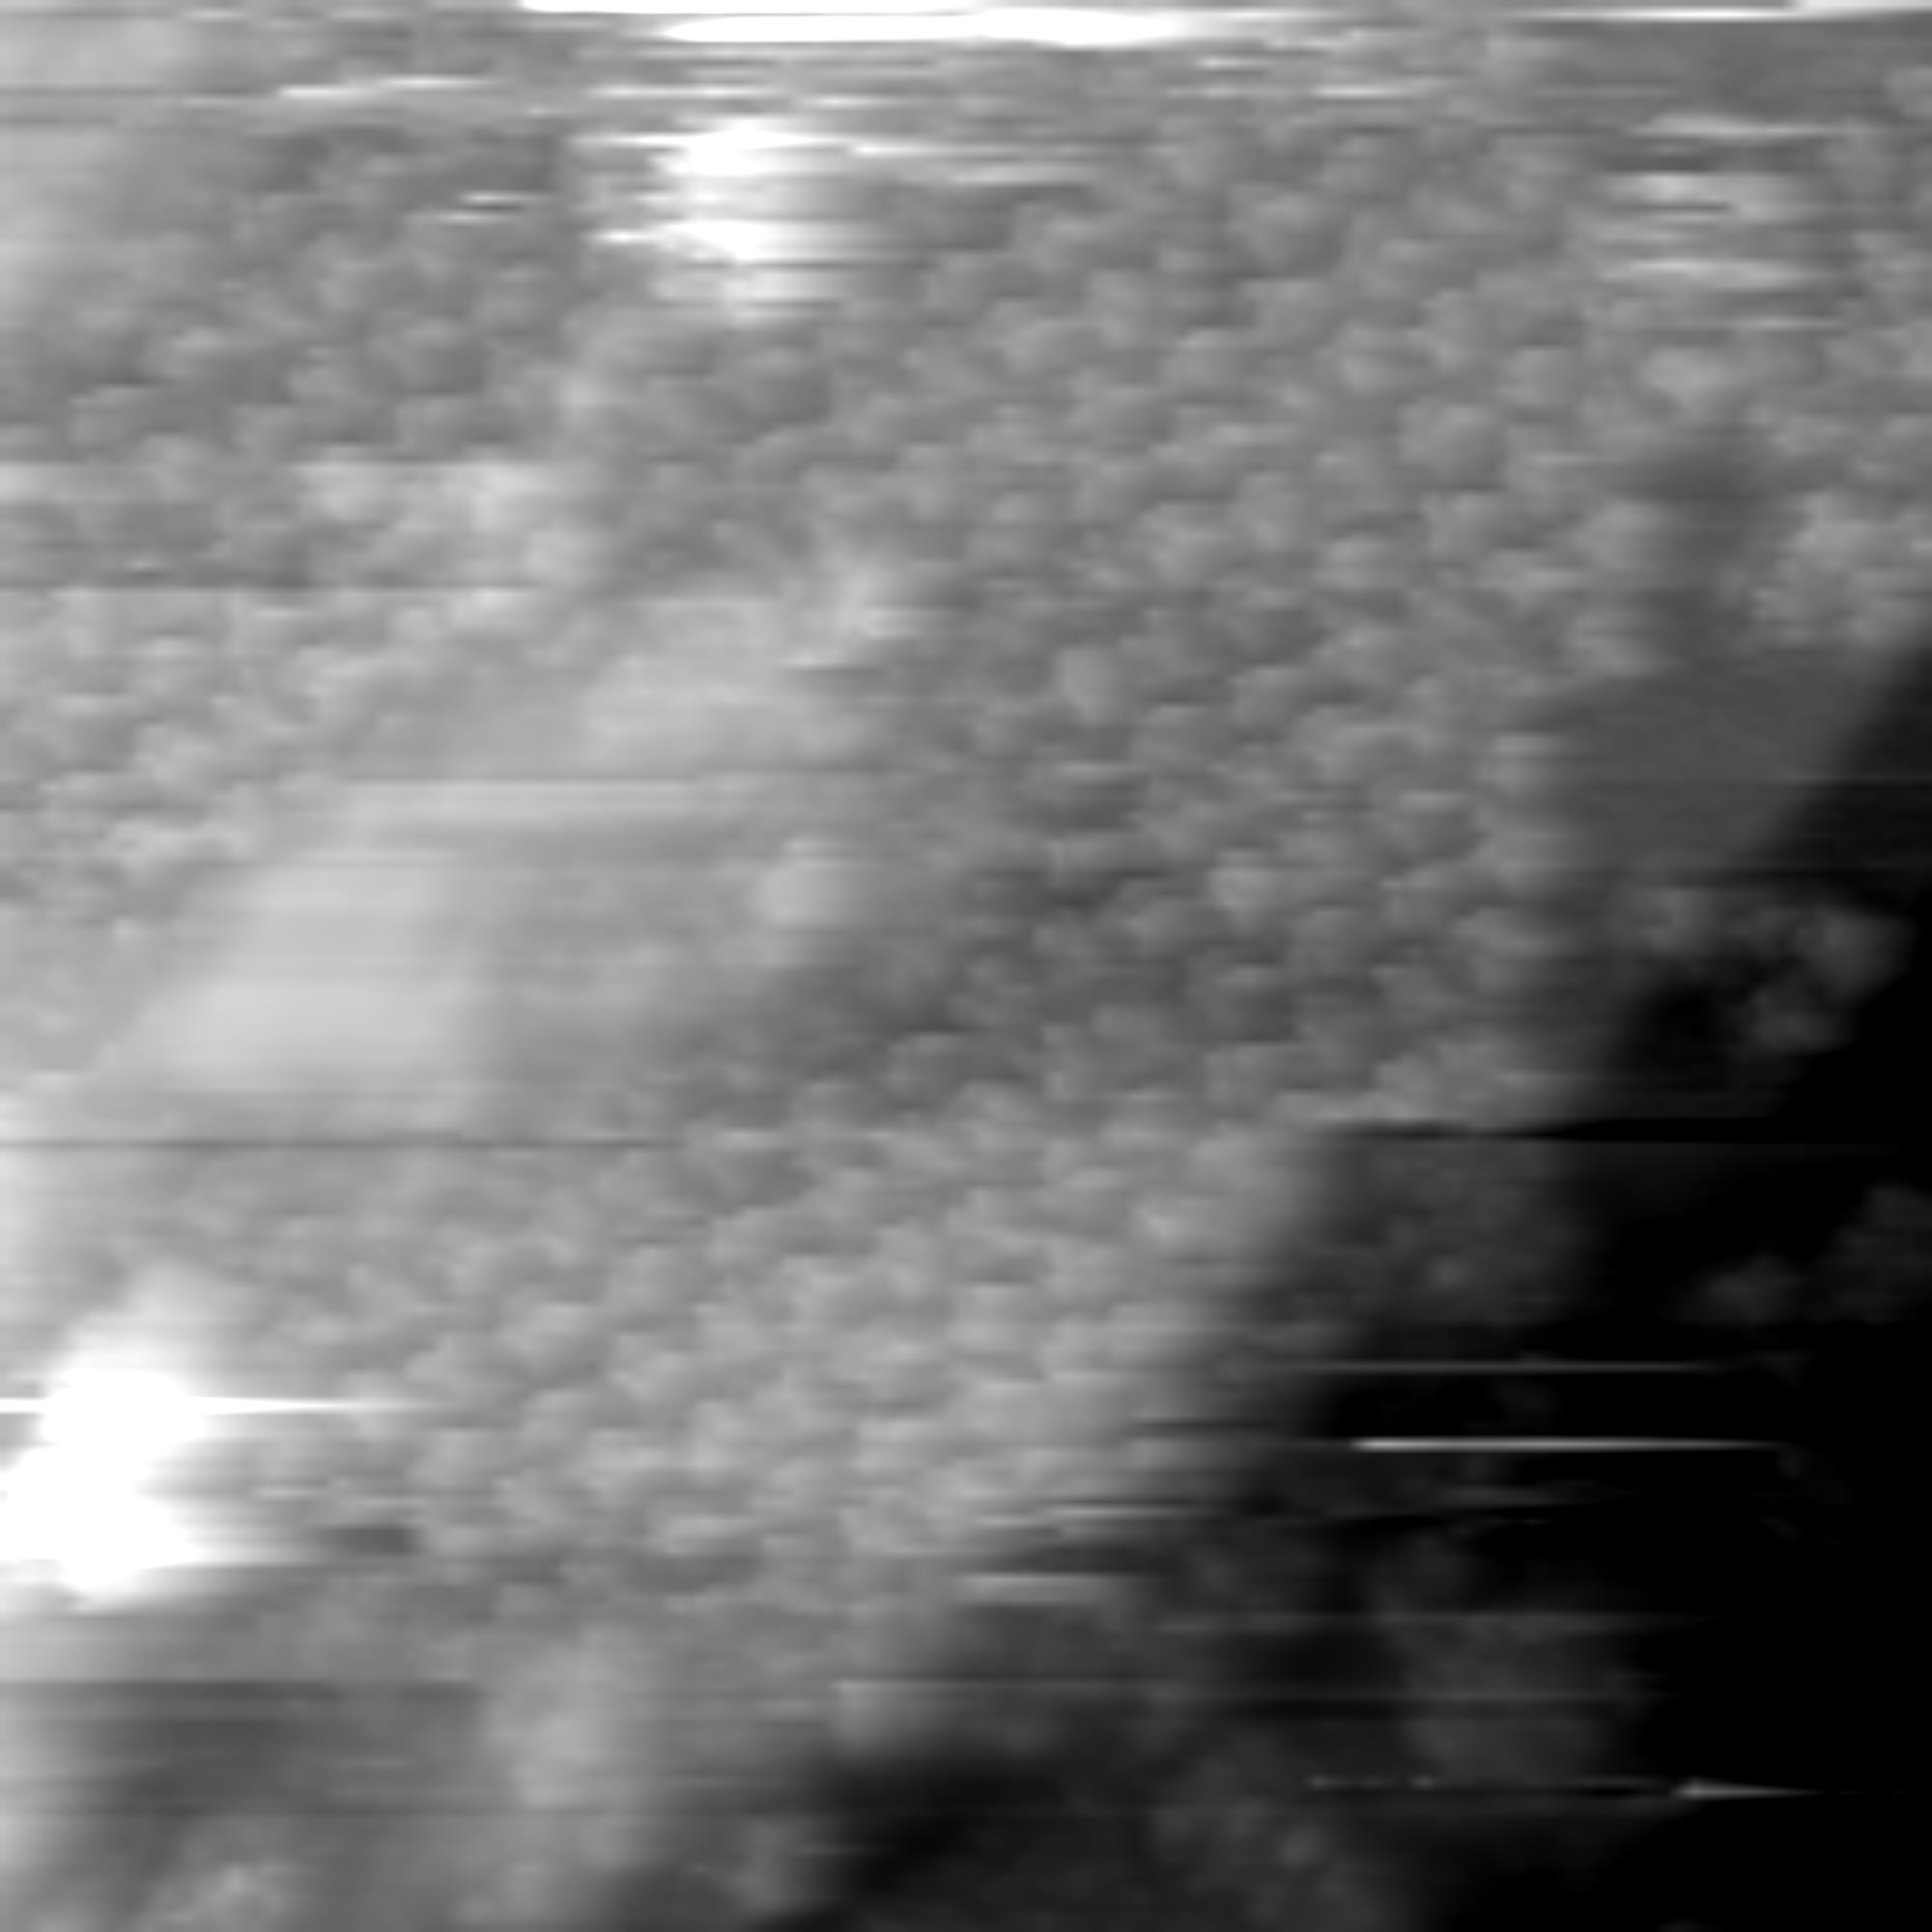
\includegraphics[width=0.5\textwidth]{./images/F151007-112800}
	\caption{TBP on Ag(100) showing some ordering}
	\label{fig:hex-TBP-Ag100}
\end{figure}

%%%%%%%%%%%%%%%%%%%%%%%%%%%%%%%%%%%%%%%%%%%%%%%%%%%%%%%%%%%%%%%%%%%%%%%%%%%%%%%%%%%%%%%%%%%%%%%%%%%